% ===================================================================
%  Week 13 — Convolutional Neural Networks
%  Session 2 of 2: Training the CNN, and when it wins
% ===================================================================
\documentclass[10pt,aspectratio=169]{beamer}
% ===================================================================
%  Shared Beamer preamble for "Practical Image Processing"
%  English slides. Compile with pdfLaTeX.
% ===================================================================

\usetheme{metropolis}
\usepackage[T1]{fontenc}
\usepackage[utf8]{inputenc}
\usepackage{lmodern}
\usepackage{listings}
\usepackage{tcolorbox}
\usepackage{fontawesome5}
\usepackage{booktabs}
\usepackage{amsmath,amssymb}
\usepackage{tikz}
\usepackage{pgfplots}
\pgfplotsset{compat=1.17}
\usetikzlibrary{arrows.meta,positioning,shapes.geometric,fit,backgrounds,matrix}
\tcbuselibrary{skins,breakable}

% ---- Palette --------------------------------------------------------
\definecolor{coursePrimary}{HTML}{1B4965}   % deep blue
\definecolor{courseAccent}{HTML}{E76F51}    % coral
\definecolor{courseGood}{HTML}{2A9D8F}      % teal
\definecolor{courseBad}{HTML}{C0392B}       % red
\definecolor{courseInfo}{HTML}{2980B9}      % blue
\definecolor{codeBg}{HTML}{F5F6FA}
\definecolor{codeKw}{HTML}{8E44AD}
\definecolor{codeStr}{HTML}{2A9D8F}
\definecolor{codeCom}{HTML}{7F8C8D}

\setbeamercolor{frametitle}{bg=coursePrimary}
\setbeamercolor{progress bar}{fg=courseAccent}
\setbeamercolor{alerted text}{fg=courseAccent}
\metroset{block=fill,sectionpage=progressbar,numbering=fraction}

% ---- Code listings (Python is built into listings) -----------------
\lstdefinestyle{course}{
  backgroundcolor=\color{codeBg},
  basicstyle=\ttfamily\scriptsize,
  keywordstyle=\color{codeKw}\bfseries,
  stringstyle=\color{codeStr},
  commentstyle=\color{codeCom}\itshape,
  numberstyle=\tiny\color{codeCom},
  numbers=left, numbersep=6pt,
  showstringspaces=false, breaklines=true, breakatwhitespace=true,
  tabsize=4, columns=fullflexible,
  frame=single, framesep=4pt, rulecolor=\color{gray!30},
  keepspaces=true, upquote=true, language=Python,
}
\lstset{style=course}
\lstdefinelanguage{bash}{
  keywords={cd,pip,python,venv,source,import}, sensitive=true,
  morecomment=[l]{\#}, morestring=[b]', morestring=[b]",
}

% ---- Reusable callout boxes ----------------------------------------
\newtcolorbox{goodbox}[1][Good practice]{colback=courseGood!8,colframe=courseGood,
  fonttitle=\bfseries,title={\faCheck~#1},boxrule=0.6pt,left=4pt,right=4pt,top=3pt,bottom=3pt}
\newtcolorbox{badbox}[1][Pitfall]{colback=courseBad!8,colframe=courseBad,
  fonttitle=\bfseries,title={\faTimes~#1},boxrule=0.6pt,left=4pt,right=4pt,top=3pt,bottom=3pt}
\newtcolorbox{infobox}[1][Note]{colback=courseInfo!8,colframe=courseInfo,
  fonttitle=\bfseries,title={\faInfoCircle~#1},boxrule=0.6pt,left=4pt,right=4pt,top=3pt,bottom=3pt}
\newtcolorbox{mathbox}[1][Math]{colback=coursePrimary!6,colframe=coursePrimary,
  fonttitle=\bfseries,title={\faCalculator~#1},boxrule=0.6pt,left=4pt,right=4pt,top=3pt,bottom=3pt}

\newcommand{\keyidea}[1]{\begin{alertblock}{Key idea}#1\end{alertblock}}
\newcommand{\term}[1]{\textbf{\color{coursePrimary}#1}}
\newcommand{\code}[1]{\lstinline[basicstyle=\ttfamily\small]|#1|}

% ---- A helper to draw a small pixel grid, cells shaded by value ----
% \pixelgrid{ {10,20,120,200,240}, {30,60,130,180,230}, ... }
\newcommand{\pixelgrid}[1]{%
  \begin{tikzpicture}[font=\scriptsize,scale=0.6]
    \foreach \row [count=\ry] in {#1} {
      \foreach \val [count=\cx] in \row {
        \draw[gray,fill=coursePrimary!8] (\cx,-\ry) rectangle ++(1,-1);
        \node at (\cx+0.5,-\ry-0.5) {\val};
      }
    }
  \end{tikzpicture}}


\title{Convolutional Neural Networks}
\subtitle{Week 13 — Session 2: Training the filters, and when CNNs win}
\author{Practical Image Processing}
\date{Lecture 13.2 \textbullet\ 60--70 min}

\begin{document}

\maketitle

\begin{frame}{Recap of Session 1}
  \begin{columns}[T]
    \begin{column}{0.58\textwidth}
      \begin{itemize}
        \item A \term{convolutional layer} = convolution with \emph{learned} filters (weight sharing).
        \item CNN recipe: Conv $\rightarrow$ ReLU $\rightarrow$ Pool, stacked, ending in FC + softmax.
        \item Our digit net: $8\times8 \rightarrow$ two conv blocks $\rightarrow$ 10 scores, $\sim$1{,}900 parameters.
        \item We can trace shapes and count params --- but the filters are still \emph{random}.
      \end{itemize}
    \end{column}
    \begin{column}{0.42\textwidth}
      \begin{alertblock}{Today's job}
        Turn random filters into good detectors --- \term{train} the net --- and judge honestly when a CNN is worth it.
      \end{alertblock}
    \end{column}
  \end{columns}
\end{frame}

\begin{frame}{Roadmap --- Session 2}\tableofcontents\end{frame}

% ==================================================================
\section{Training a CNN}
% ==================================================================

\begin{frame}{How does it learn the filters?}
  \begin{enumerate}
    \item \term{Forward pass}: run an image through; get predicted probabilities.
    \item \term{Loss}: measure how wrong (\term{cross-entropy} between prediction and true label).
    \item \term{Backprop}: compute how each weight affected the loss (the gradient).
    \item \term{Update}: nudge every weight to reduce the loss (\term{gradient descent}).
  \end{enumerate}
  \keyidea{Repeat over many images and epochs; the filters gradually become good detectors.}
\end{frame}

\begin{frame}{The forward pass, concretely}
  \begin{center}
  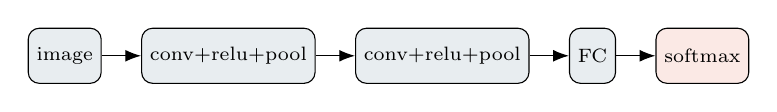
\begin{tikzpicture}[font=\scriptsize,node distance=6mm and 5mm,
      box/.style={draw,rounded corners,fill=coursePrimary!10,minimum height=7mm,inner sep=3pt}]
    \node[box] (img) {image};
    \node[box,right=of img] (c1) {conv+relu+pool};
    \node[box,right=of c1] (c2) {conv+relu+pool};
    \node[box,right=of c2] (fc) {FC};
    \node[box,right=of fc,fill=courseAccent!15] (sm) {softmax};
    \draw[-{Latex[length=2mm]}] (img)--(c1);
    \draw[-{Latex[length=2mm]}] (c1)--(c2);
    \draw[-{Latex[length=2mm]}] (c2)--(fc);
    \draw[-{Latex[length=2mm]}] (fc)--(sm);
  \end{tikzpicture}
  \end{center}
  \begin{itemize}
    \item Data flows left-to-right; the output is 10 probabilities.
    \item Nothing changes during a forward pass --- it is pure prediction.
    \item Learning happens on the way \emph{back}, once we know how wrong we were.
  \end{itemize}
\end{frame}

\begin{frame}{Softmax with real numbers}
  Suppose the FC layer outputs logits $z = (2.0,\ 0.5,\ -1.0)$ for three classes.
  \begin{mathbox}[Exponentiate, then normalize]
    $e^{2.0}=7.39,\quad e^{0.5}=1.65,\quad e^{-1.0}=0.37$\\[3pt]
    sum $=9.41 \Rightarrow p=(0.79,\ 0.18,\ 0.04)$
  \end{mathbox}
  \begin{itemize}
    \item Biggest logit $\rightarrow$ biggest probability; everything stays in $[0,1]$ and sums to 1.
    \item Softmax is monotone: it never changes \emph{which} class wins, only the confidence.
  \end{itemize}
\end{frame}

\begin{frame}{Cross-entropy loss, intuitively}
  \begin{itemize}
    \item The network outputs a probability for each class. Cross-entropy is low when it puts high
          probability on the \emph{correct} class.
    \item Confidently wrong $\rightarrow$ huge loss. Correct and confident $\rightarrow$ near-zero loss.
    \item Training minimizes the average loss over the data.
  \end{itemize}
  \begin{mathbox}
    Loss for one sample $= -\log(p_{\text{true class}})$. Push $p_{\text{true}}\to 1$.
  \end{mathbox}
\end{frame}

\begin{frame}{Cross-entropy, with real numbers}
  Same example: predicted $p=(0.79,0.18,0.04)$. Loss depends only on the \emph{true} class.
  \begin{center}
  \begin{tabular}{@{}lcc@{}}
    \toprule
    \textbf{True class} & $p_{\text{true}}$ & \textbf{Loss} $=-\log p_{\text{true}}$ \\
    \midrule
    class 0 (right, confident) & 0.79 & 0.24 \\
    class 1 (partly right)     & 0.18 & 1.71 \\
    class 2 (confidently wrong)& 0.04 & 3.22 \\
    \bottomrule
  \end{tabular}
  \end{center}
  \begin{itemize}
    \item The more probability we gave the \emph{true} class, the smaller the loss.
    \item Being confidently wrong is punished hard --- that steep penalty drives learning.
  \end{itemize}
\end{frame}

\begin{frame}{Backprop and gradient descent}
  \begin{itemize}
    \item \term{Backprop} applies the chain rule to get $\partial \text{Loss}/\partial w$ for every weight $w$.
    \item The gradient says: ``increase this weight $\rightarrow$ loss goes up/down, this much.''
    \item \term{Gradient descent} then steps every weight the opposite way.
  \end{itemize}
  \begin{mathbox}[The update rule]
    $\displaystyle w \leftarrow w - \eta\,\frac{\partial \text{Loss}}{\partial w}$ \qquad ($\eta$ = learning rate)
  \end{mathbox}
  \keyidea{Backprop finds the direction; the learning rate sets the step. Repeat millions of times.}
\end{frame}

\begin{frame}{Mini-batches, epochs, learning rate}
  \begin{itemize}
    \item \term{Mini-batch}: update on a small group of images at a time (we used 128) --- faster, smoother.
    \item \term{Epoch}: one full pass over the training set. We ran 60.
    \item \term{Learning rate}: step size of each update. Too big $\rightarrow$ diverges; too small $\rightarrow$ crawls.
  \end{itemize}
  \begin{badbox}
    Most training failures are a bad learning rate. If loss explodes or won't move, change it first.
  \end{badbox}
\end{frame}

\begin{frame}{Learning rate: too small, right, too big}
  \begin{center}
  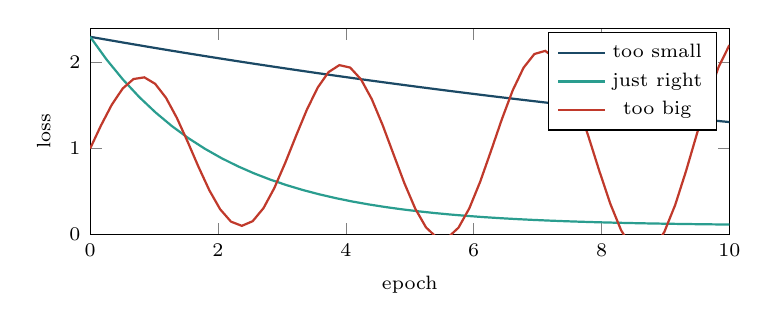
\begin{tikzpicture}
    \begin{axis}[width=0.8\linewidth,height=4.2cm,xlabel={epoch},ylabel={loss},
        legend style={font=\scriptsize,at={(0.98,0.98)},anchor=north east},
        tick label style={font=\scriptsize},label style={font=\scriptsize},
        ymin=0,ymax=2.4,xmin=0,xmax=10]
      \addplot[coursePrimary,thick,domain=0:10,samples=40] {2.2*exp(-0.06*x)+0.1};
      \addplot[courseGood,thick,domain=0:10,samples=40] {2.2*exp(-0.5*x)+0.1};
      \addplot[courseBad,thick,domain=0:10,samples=60] {1.0+0.8*sin(deg(2*x))*exp(0.05*x)};
      \legend{too small,just right,too big}
    \end{axis}
  \end{tikzpicture}
  \end{center}
  Blue crawls, green drops fast and settles, red oscillates and diverges. Tune $\eta$ first.
\end{frame}

\begin{frame}{Training in action}
  \begin{columns}[T]
    \begin{column}{0.55\textwidth}\begin{center}
      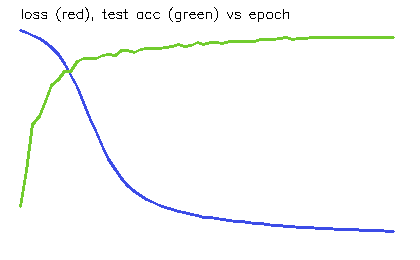
\includegraphics[width=0.98\linewidth]{../assets/training_curve.png}
    \end{center}\end{column}
    \begin{column}{0.45\textwidth}
      \begin{itemize}
        \item Red: training loss falls each epoch.
        \item Green: test accuracy climbs, then plateaus near 0.97.
        \item Watching both curves is how you spot under/over-fitting live.
      \end{itemize}
    \end{column}
  \end{columns}
\end{frame}

% ==================================================================
\section{Results}
% ==================================================================

\begin{frame}{Reading digits --- the DocScan payoff}
  \begin{center}
  
\includegraphics[width=0.82\linewidth]{../assets/predictions.png}
  \end{center}
  \vspace{2pt}
  Test digits with the CNN's prediction (green = correct). This is the meter-digit reader DocScan needs.
\end{frame}

\begin{frame}{CNN vs classical --- an honest comparison}
  \begin{center}
  \begin{tabular}{@{}lc@{}}
    \toprule
    \textbf{Method} & \textbf{Test accuracy (digits)} \\
    \midrule
    CNN (learned filters) & 0.97 \\
    SVM on raw pixels & 0.99 \\
    \bottomrule
  \end{tabular}
  \end{center}
  \begin{itemize}
    \item On \emph{easy}, clean $8\times8$ digits, classical ML is already excellent --- CNN isn't magic here.
    \item The CNN's real advantage shows on \emph{hard, large, varied} images --- and with \term{transfer learning} (Week 14).
  \end{itemize}
\end{frame}

\begin{frame}{When do CNNs really win?}
  \begin{itemize}
    \item Large, varied datasets where hand features can't capture the variation.
    \item Problems where the useful features are unknown (the network discovers them).
    \item Recall Week 12: HOG+SVM plateaued at 48\% on look-alike cars --- that's where learned features help.
  \end{itemize}
  \keyidea{Small clean problem $\rightarrow$ classical is fine. Big messy problem $\rightarrow$ deep learning pulls ahead.}
\end{frame}

% ==================================================================
\section{Deep dive}
% ==================================================================

\begin{frame}{The feature hierarchy}
  \begin{itemize}
    \item Layer 1: edges and simple strokes (like the learned filters we saw).
    \item Layer 2--3: corners, curves, digit parts (loops, junctions).
    \item Deeper: whole-shape detectors that fire for a specific digit.
  \end{itemize}
  \keyidea{A CNN builds complexity gradually --- simple parts combine into meaningful wholes, all learned.}
\end{frame}

\begin{frame}{Overfitting vs underfitting}
  \begin{center}
  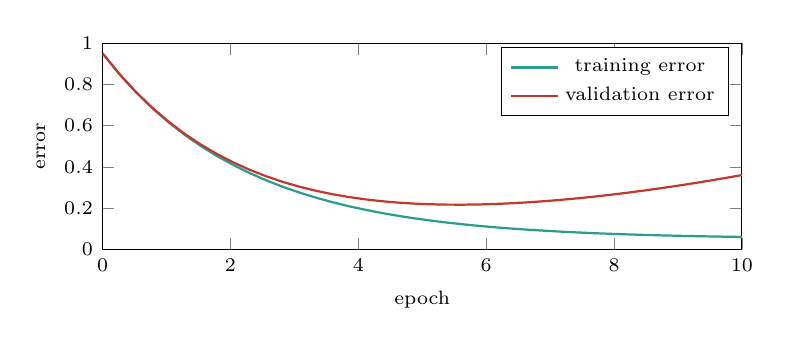
\begin{tikzpicture}
    \begin{axis}[width=0.8\linewidth,height=4.2cm,xlabel={epoch},ylabel={error},
        legend style={font=\scriptsize,at={(0.98,0.98)},anchor=north east},
        tick label style={font=\scriptsize},label style={font=\scriptsize},
        ymin=0,ymax=1,xmin=0,xmax=10]
      \addplot[courseGood,thick,domain=0:10,samples=40] {0.9*exp(-0.45*x)+0.05};
      \addplot[courseBad,thick,domain=0:10,samples=40] {0.9*exp(-0.45*x)+0.05+0.03*x*x/10};
      \legend{training error,validation error}
    \end{axis}
  \end{tikzpicture}
  \end{center}
  \begin{itemize}
    \item Training error keeps dropping; validation error turns \emph{up} --- classic \term{overfitting}.
    \item Stop where validation is lowest (\term{early stopping}); if \emph{both} stay high, you \term{underfit}.
  \end{itemize}
\end{frame}

\begin{frame}{Regularization: keeping CNNs honest}
  \begin{itemize}
    \item CNNs have many parameters $\rightarrow$ they can overfit (Week 12's lesson returns).
    \item \term{Dropout}: randomly zero some activations during training so the net can't rely on any one.
    \item \term{Data augmentation}: random shifts/rotations of training images --- free extra data, more invariance.
    \item \term{Weight decay}: penalize large weights to keep the model simple.
  \end{itemize}
\end{frame}

\begin{frame}{Data augmentation, concretely}
  \begin{columns}[T]
    \begin{column}{0.5\textwidth}
      \begin{itemize}
        \item Take each training digit and make cheap variants: shift 1px, rotate a few degrees, add noise.
        \item The label stays the same --- a shifted ``7'' is still a 7.
        \item The net sees more variation $\rightarrow$ learns invariance for free.
      \end{itemize}
    \end{column}
    \begin{column}{0.5\textwidth}
      \begin{goodbox}[Cheap and effective]
        On small datasets (like our meter digits), augmentation is often the single biggest accuracy win --- before you reach for a bigger model.
      \end{goodbox}
    \end{column}
  \end{columns}
\end{frame}

\begin{frame}{Why CNNs need a GPU (and lots of data)}
  \begin{itemize}
    \item Millions of multiply-adds per image; a GPU does them massively in parallel.
    \item Deep nets have millions of parameters --- they need many examples to fit without overfitting.
    \item Our digit net is tiny and trains in seconds; ImageNet-scale nets train for days.
  \end{itemize}
  \begin{goodbox}
    Small data + deep net = overfitting. Next week's \term{transfer learning} fixes exactly this.
  \end{goodbox}
\end{frame}

\begin{frame}[fragile]{A CNN in PyTorch}
\begin{lstlisting}[language=Python]
class DigitCNN(nn.Module):
    def __init__(self):
        super().__init__()
        self.c1 = nn.Conv2d(1, 8, 3, padding=1)
        self.c2 = nn.Conv2d(8, 16, 3, padding=1)
        self.pool = nn.MaxPool2d(2)
        self.fc = nn.Linear(16*2*2, 10)
    def forward(self, x):
        x = self.pool(torch.relu(self.c1(x)))
        x = self.pool(torch.relu(self.c2(x)))
        return self.fc(x.flatten(1))
\end{lstlisting}
  Conv $\rightarrow$ ReLU $\rightarrow$ Pool, twice, then a linear classifier. That is the whole digit reader.
\end{frame}

\begin{frame}[fragile]{Reading the model, line by line}
\begin{lstlisting}[language=Python]
self.c1 = nn.Conv2d(1, 8, 3, padding=1)   # 1 -> 8 maps, keep 8x8
self.pool = nn.MaxPool2d(2)               # halve H and W
self.fc = nn.Linear(16*2*2, 10)           # 64 features -> 10 logits
\end{lstlisting}
  \begin{itemize}
    \item \code{Conv2d(1,8,3,padding=1)}: matches Session 1's shape table exactly.
    \item \code{16*2*2 = 64}: the flattened size after two pools --- if this number is wrong, the net won't build.
    \item \code{forward} just chains the blocks; \code{flatten(1)} keeps the batch dimension.
  \end{itemize}
  \begin{badbox}
    A mismatched \code{Linear} input size is the \#1 first-run CNN error. Compute it from the shape table.
  \end{badbox}
\end{frame}

\begin{frame}[fragile]{The training loop}
\begin{lstlisting}[language=Python]
opt = torch.optim.Adam(net.parameters(), lr=1e-3)
loss_fn = nn.CrossEntropyLoss()
for epoch in range(60):
    for xb, yb in train_loader:      # mini-batches of 128
        opt.zero_grad()              # clear old gradients
        logits = net(xb)             # forward pass
        loss = loss_fn(logits, yb)   # cross-entropy
        loss.backward()              # backprop: fill gradients
        opt.step()                   # gradient-descent update
\end{lstlisting}
  \begin{itemize}
    \item Every line maps to a step from the first training slide: forward, loss, backprop, update.
    \item \code{CrossEntropyLoss} does softmax + $-\log p_{\text{true}}$ in one call.
    \item Forgetting \code{zero\_grad()} silently accumulates gradients --- a classic bug.
  \end{itemize}
\end{frame}

% ==================================================================
\section{In-class exercise}
% ==================================================================

\begin{frame}{\faPen~In-class exercise (10 min)}
  \begin{infobox}[Reason about training]
  \end{infobox}
  \begin{enumerate}
    \item The true class has predicted probability 0.5. What is the cross-entropy loss? (use $-\log$)
    \item Training loss keeps falling but validation accuracy drops. What is happening, and one fix?
    \item Our CNN got 0.97 and the SVM 0.99 on digits. Does that mean CNNs are worse? Explain.
    \item You forgot \code{opt.zero\_grad()} in the loop. What goes wrong?
  \end{enumerate}
\end{frame}

\begin{frame}{\faPen~Debrief}
  \begin{itemize}
    \item (1) $-\log(0.5) \approx 0.69$ --- ``half sure of the right answer'' costs about 0.69 nats.
    \item (2) \term{Overfitting}; fix with early stopping, dropout, weight decay, or data augmentation.
    \item (3) No --- on easy clean data classical ML is already near-perfect; CNNs win on hard, varied,
          large-scale data and via transfer learning.
    \item (4) Gradients from every batch accumulate, so each update uses a corrupted, oversized gradient.
  \end{itemize}
  \keyidea{Match the tool to the problem --- and remember the loop's four steps and their pitfalls.}
\end{frame}

% ==================================================================
\section{Wrap-up}
% ==================================================================

\begin{frame}{What you should now be able to do}
  \begin{itemize}
    \item Explain a CNN as convolution with \emph{learned} filters, plus ReLU, pooling, and a classifier.
    \item Describe how training works: forward, loss, backprop, gradient descent --- with numbers.
    \item Read training curves and recognize the role of batches, epochs, learning rate, regularization.
    \item Judge honestly when a CNN beats classical ML --- and when it doesn't.
  \end{itemize}
\end{frame}

\begin{frame}{This week's deliverable}
  \begin{alertblock}{Due before Week 14 (see \code{project/})}
    \begin{enumerate}
      \item Train the small digit CNN; report test accuracy and show the training curve.
      \item Visualize the learned first-layer filters; describe what they detect.
      \item Compare to a classical baseline (SVM/k-NN) on the same digits.
      \item Add one regularizer (dropout or augmentation) and report its effect on validation accuracy.
      \item Reflect: on your data, when would you expect a CNN to beat classical features?
    \end{enumerate}
  \end{alertblock}
\end{frame}

\begin{frame}[standout]
  A CNN learns the filters Week 3 made us design.\\[4pt]
  \normalsize Convolution + ReLU + pooling, trained end to end --- features and classifier together.
\end{frame}

\end{document}
